\documentclass[]{article}

\usepackage{tikz}
\usepackage{amsmath}
\usepackage{amsfonts}
\usepackage{amssymb}
\usepackage{tkz-base}
\usepackage{tkz-euclide}
\usepackage{xcolor}
\usepackage{pgfplots}
\usepackage{graphicx}
\usepackage{url}

% Required package
\usetikzlibrary{positioning}
\usetikzlibrary{svg.path}
\usetikzlibrary{arrows}
\usetikzlibrary{shapes.geometric,calc}

\newdimen\XCoord
\newdimen\YCoord
\newcommand*{\ExtractCoordinate}[1]{\path (#1); \pgfgetlastxy{\XCoord}{\YCoord};}%

%opening
\title{Impedance Control,\\a.k.a. ``Direct'' Compliance Control}
\author{Glen Henshaw}

\begin{document}

\maketitle

\section{Intro}
Last time we discussed ``indirect'' compliance control, a scheme whereby we enforced a desired tradeoff between force and position at the end effector by calculating the reaction of a fictional spring--mass--damper system to the sensed forces we are currently seeing, and then commanding an inner position control loop to mimic that reaction. This is called ``indirect'' because the inner position loop indirectly causes the robot arm to be compliant. Indirect compliance control is also known as admittance control, admittance being the technical term for the the motion that results from a force. Admittance control is good for presenting a relatively stiff system to the environment, but can become unstable as the system is tuned to become more compliant.

The dual approach to admittance control is impedance control, ``impedance'' referring to the amount of force that results from a velocity input. Impedance controllers do an excellent job or presenting a very compliant robot to the environment, and become unstable as the amount of compliance is decreased.

We also talked about the Salisbury stiffness controller (a bit dismissively!) This control law is a simple form of impedance control. Let's recap it here.
\pagebreak

\subsection{Time warp to last lecture: the Salisbury Stiffness Controller}

Here's a spring--mass--damper system:
\begin{figure}[h!]
\centering
 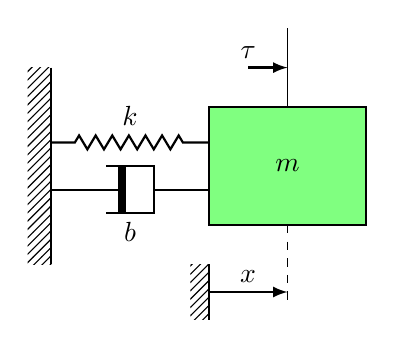
\begin{tikzpicture}[every node/.style={outer sep=0pt},thick,
 mass/.style={draw,thick},
 spring/.style={thick,decorate,decoration={zigzag,pre length=0.3cm,post
 length=0.3cm,segment length=6}},
 ground/.style={fill,pattern=north east lines,draw=none,minimum
 width=0.75cm,minimum height=0.3cm},
 dampic/.pic={\fill[white] (-0.1,-0.3) rectangle (0.3,0.3);
 \draw (-0.3,0.3) -| (0.3,-0.3) -- (-0.3,-0.3);
 \draw[line width=1mm] (-0.1,-0.3) -- (-0.1,0.3);}]

  \node[mass,minimum width=2cm,minimum height=1.5cm,fill=green!50] (m1) {$m$};
   \node[left=2cm of m1,ground,minimum width=3mm,minimum height=2.5cm] (g1){};
  \draw (g1.north east) -- (g1.south east);

  \draw[spring] ([yshift=3mm]g1.east) coordinate(aux)
   -- (m1.west|-aux) node[midway,above=1mm]{$k$};

  \draw ([yshift=-3mm]g1.east) coordinate(aux')
   -- (m1.west|-aux') pic[midway]{dampic} node[midway,below=3mm]{$b$};
 
  \foreach \X in {1}  
  {\draw[thin] (m\X.north) -- ++ (0,1) coordinate[midway](aux\X);
   \draw[latex-] (aux\X) -- ++ (-0.5,0) node[above]{$\tau$}; 
   \draw[thin,dashed] (m\X.south) -- ++ (0,-1) coordinate[pos=0.85](aux'\X);
   \draw[latex-] (aux'\X) -- ++ (-1,0) node[midway,above]{$x$}
    node[left,ground,minimum height=7mm,minimum width=1mm] (g'\X){};
   \draw[thick] (g'\X.north east) -- (g'\X.south east);
  }

\end{tikzpicture}
\end{figure}

Imagine what would happen if you had chosen your spring and damping gains, and then perturbed the system by exerting a force $\tau_{1}$ on it. It would move, of course, but it would do so in a way that was dependent on $k_{1}$m $b_{1}$, and $m_{1}$. This is referred to as ``mechanical impedance'', and is a measure of how much a system resists motion when a force is applied.

One very effective way of thinking about robotic contact operations is to consider how much mechanical impedance they require. With the right controller structure, we can build this in by choosing the right gains.

Suppose we just want to control the stiffness of the arm as it interacts with the environment. We want to do this around all siz axes, x--y--z and roll--pitch--yaw. In other words, we want to enforce the following:
\begin{displaymath}
 \underline{F} = K_{p_{x}} \underbrace{(x - x_{d})}_{\delta x}
\end{displaymath}
This is called ``stiffness control'' instead of ``impedance control'' because we are only specifying $K_{p}$. What controller achieves this Cartesian stiffness?

\begin{eqnarray}
 \dot{x} & = & J\dot{\theta} \cong J\ \delta\underline{\theta}\ \  \leftarrow\ \  \text{Good for small $\delta x$} \nonumber \\
 \underline{F} & = & K_{p_{x}}\ \delta\underline{x}\ \  \Rightarrow\ \  \underline{F} = K_{p_{x}}J\ \delta\underline{\theta} \nonumber \\
 \underline{\tau} & = & J^{T}\underline{F}\ \ \Rightarrow\ \ \underline{\tau} = \underbrace{J^{T}(\underline{\theta})K_{p_{x}}J(\underline{\theta})}_{K_{p\theta} (\underline{\theta})}\ \delta\underline{\theta} \nonumber
\end{eqnarray}

So a potential control law is:
\begin{displaymath}
 \underline{\tau} = \underbrace{J^{T}(\underline{\theta})K_{p_{x}}J(\underline{\theta})}_{K_{p\theta} (\underline{\theta})}\underline{\tilde{\theta}} + K_{v}\dot{\tilde{\underline{\theta}}}
\end{displaymath}
where the final term just adds some damping to make the system stable. Note that $K_{v}$ is a constant.

It's important to note that $K_{p\theta}$ is in general much much lower than the $K_{p}$ gain for a position control PD control law. This means that the Salisbury stiffness controller is much worse at rejecting disturbances than a position controller would be. We have sacrificed positional accuracy for compliance. In some sense this is unavoidable.

Of course, you could try to add a model term to a controller like this to try to at least cancel out ``disturbances'' that are a result of the manipulator dynamcis and environmental forces you can model, like gravity. There's a considerable amount of research in this area.

\section{More Advanced Impedance Controllers}
The Salisbury stiffness control has several problems that we're going to try to fix here.

One is that, typically, we don't want to present just a stiffness to the environment; we also want a controllable amount of damping and maybe inertia. In other words, we want to control all of the knobs in our virtual spring--mass--damper system, not just the stiffness knob.

Let's start with a desired dynamic equation:
\begin{equation}
 \underline{F}_{d} = M_{x} \ddot{\tilde{\underline{x}}} + K_{vx}\dot{\tilde{\underline{x}}} + K_{px}\tilde{\underline{x}}
\end{equation}
where $\tilde{\underline{x}} = \underline{x} - \underline{x}_{d}$ is the deviation of the system away from the desired trajectory $\underline{x}_{d}$.

In order to map these equations into joint space, the same trick we played when deriving the Salisbury stiffness controller, we premultiply by the Jacobian transpose:
\begin{equation}
 \tau = J^{T}(\underline{\theta})M_{x} \ddot{\tilde{\underline{x}}} + J^{T}(\underline{\theta})K_{vx}\dot{\tilde{\underline{x}}} + J^{T}(\underline{\theta})K_{px}\tilde{ \underline{x}}
\end{equation}

But we really want this in terms of joint deviations, not Cartesian deviations. So we take the partials of each term with respect to their joint space equivalents. Thus:
\begin{equation}
 K_{v} = \frac{\partial \tau}{\partial\underline{\dot{\theta}}} = \frac{\partial( J^{T}(\underline{\theta})K_{vx}\dot{\tilde{x}})}{\partial\underline{\dot{\theta}}} = J^{T}(\underline{\theta})K_{vx}J(\underline{\theta}) \label{damping}
\end{equation}
which gives us a joint--space matrix $K_{v}$ which is the equivalent to the Cartesian damping matrix $K_{vx}$. Similarly we can take the partial of the stiffness term to get:
\begin{equation}
\begin{split}
    K_{p} & = \frac{\partial \tau}{\partial\underline{\theta}} = \frac{\partial ( J^{T}(\underline{\theta})K_{px}\tilde{x})}{\partial\underline{\theta}}\\ & = J^{T}(\underline{\theta})K_{px}J(\underline{\theta}) + \frac{\partial J^{T}(\underline{\theta})K_{px}}{\partial \underline{\theta}^{T}}\tilde{\underline{x}} \label{stiffness}
\end{split}
\end{equation}
Note that the first term of Equation \ref{stiffness} is what we derived for the Salisbury stiffness controller. The second term accounts for the change of the Jacobian as the joints move. For small deviations, e.g. for systems that display high levels of stiffness, this is probably small and can be ignored. But if we want a system that displays low levels of stiffness, there is no guarantee that the joint motions will be small. Ignoring that second term will lead to ``errors'' in the mapping from Cartesian to joint stiffness, meaning that the system will not continue to display the desired Cartesian stiffness.

The purists among you may note that technically we should have \textit{also} taken the partial of $K_{vx}$ with respect to $\underline{\theta}$, which would have added a third term, e.g.
\begin{equation}
 \begin{split}
    K_{p} & = \frac{\partial \tau}{\partial\underline{\theta}} = \frac{\partial ( J^{T}(\underline{\theta})K_{px}\tilde{\theta} + J^{T}(\underline{\theta})K_{vx}\dot{\tilde{\theta}})}{\partial\underline{\theta}}\\ & = J^{T}(\underline{\theta})K_{px}J(\underline{\theta}) + \frac{\partial J^{T}(\underline{\theta})}{\partial \underline{\theta}^{T})}K_{px}\tilde{\underline{x}} + \frac{\partial J^{T}(\underline{\theta})}{\partial\underline{\theta}}K_{vx}\dot{\underline{x}}
 \end{split}
\end{equation}
which would actually add a term to the equivalent damping, e.g.
\begin{equation}
 K_{v} = J^{T}(\underline{\theta})K_{vx}J(\underline{\theta}) + \frac{\partial J^{T}(\underline{\theta})}{\partial\underline{\theta}}K_{vx}\dot{\underline{x}}
\end{equation}
which would correspond to a change in the damping matrix as the joints move. However, in most popular implementations I know of this term is generally omitted (see, for instance, the derivation by Hirzinger and Albu--Sch\"affer in the references). For that matter, we could also have taken the partial with respect to $\underline{\ddot{\theta}}$ to derive an inertia term. This is rarely done because it would require feeding back the actual joint acceleration, which is problematic to estimate unless you have accelerometers on your robot. But it has been done, and can be used to make a robot (or, more commonly, a haptic device) present an inertia to the environment that is different from the  system inertia.

In practice, there are many variations on the theme of which terms to include and which to ignore. They mostly all ``work'', as long as you are intelligent about what the effects of including or excluding specific terms are.

So our impedance control implementation then becomes
\begin{equation}
 \tau_{d} = K_{p}(\underline{\theta}_{d} - \underline{\theta}) + K_{v}(\dot{\underline{\theta}}_{d} - \dot{\underline{\theta}}) \label{impedancecontrol}
\end{equation}
where $\underline{\theta}_{d}, \dot{\underline{\theta}}_{d}$ must be calculated using inverse kinematics from the desired Cartesian trajectory $\underline{x}_{d}, \dot{\underline{x}}_{d}$. In practice the $\dot{\underline{\theta}}_{d}$ term is often omitted.

Note, however, that notwithstanding the terms containing the partials of the Jacobian, it is still true that the performance of this control law will vary as the joints move around. The reason for this is of course that we made an assumption in taking the partials:
\begin{displaymath}
    \frac{\partial K_{px}\tilde{\underline{x}}}{\partial \underline{\theta}} = K_{px}J(\underline{\theta})
\end{displaymath}
is only valid when $\tilde{\underline{x}}$ is small. In order to make this really work, you have to continually re--evaluate $K_{p}$ and $K_{v}$ in light of the current arm pose. As mentioned in the last lecture, the loop rates for good compliance control implementations often want to be many hundreds to thousands of Hertz, and depending on the computing resources at your disposal, re--evaluating these matrices at the required rate may be a significant burden. There are lots of schemes that play with what terms get evaluated at what rates.

\section{Joint torques???}
We also stated last time that the Salisbury stiffness controller ignored the natural arm dynamics. You'll note that we didn't address those here either. So if you stick the controller derived in Equation \ref{impedancecontrol} into the Hamiltonian manipulator dynamics
\begin{displaymath}
 M(\underline{\theta})\ddot{\underline{\theta}} + C(\underline{\theta}, \dot{\underline{\theta}}) + E(\underline{\theta}, \dot{\underline{\theta}}) = \underline{\tau}
\end{displaymath}
you get
\begin{equation}
 M(\underline{\theta})\ddot{\underline{\theta}} + C(\underline{\theta}, \dot{\underline{\theta}}) + E(\underline{\theta}, \dot{\underline{\theta}}) = K_{p}(\underline{\theta}_{d} - \underline{\theta}) + K_{v}(\dot{\underline{\theta}}_{d} - \dot{\underline{\theta}})
\end{equation}
which looks suspiciously like a linear joint control scheme. And in fact that's what this is: you're just doing linear (or quasi--linear) PD joint control with low PD gains, with all of the problems that implies. If our joint rates were small, maybe that wouldn't be a problem, but the entire goal of impedance control (versus admittance control) is to respond \textit{quickly} to environmental forces, so this is maybe not the best assumption to make.

One intelligent thing to do would be to apply $\alpha-\beta$ partitioning to try to improve the performance, e.g. change the control law from Equation \ref{impedancecontrol} to something like
\begin{equation}
 \tau = M(\underline{\theta})\left(\ddot{\underline{\theta}}_{d} + K_{p}(\underline{\theta}_{d} - \underline{\theta}) + K_{v}(\dot{\underline{\theta}}_{d} - \dot{\underline{\theta}})\right) + C(\underline{\theta}, \dot{\underline{\theta}}) + E(\underline{\theta}, \dot{\underline{\theta}})
\end{equation}
and there are indeed people who do it this way. Of course, this just adds even more demands on your poor overloaded embedded computer, because all of this still needs to be run at up to a couple of kilohertz, now including the recursive Newton--Euler scheme you have to use to calculate the forward dynamics.

Here is a block diagram of what this implementation looks like:
\begin{figure}[h!]
 \centering
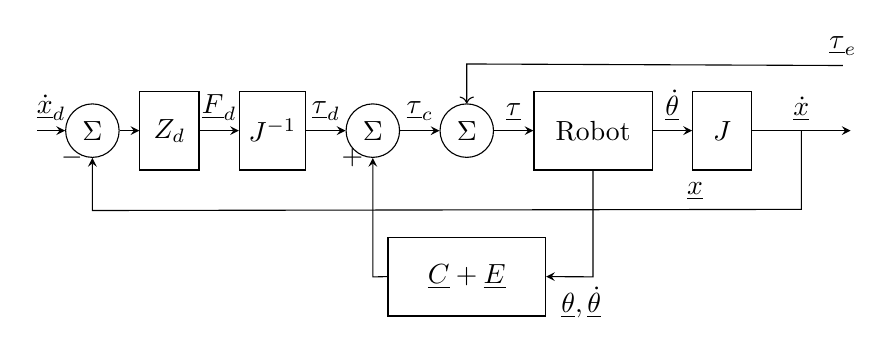
\begin{tikzpicture}
 % Sum shape
 \node[circle,draw, minimum width=0.5cm] (sum) at (-1,0){$\Sigma$} ;
 \node[draw,minimum height=1cm, minimum width=0.75cm, right=0.25cm of sum] (Zd) {$Z_{d}$};
 
 % Controller
\node [draw,
    minimum width=0.5cm,
    minimum height=1cm,
    right=0.5cm of Zd
]  (Jinv) {$J^{-1}$};

 \node[circle, draw, 
        minimum width=0.5cm,
        right=0.5cm of Jinv
        ] (sum2) {$\Sigma$};

\node[circle, draw,
    minimum width=0.5,
    right=0.5cm of sum2
    ] (sum3) {$\Sigma$};
    
 
% System H(s)
\node [draw,
    minimum width=1.5cm, 
    minimum height=1cm,
    right=0.5cm of sum3
] (robot) {Robot};

\node [draw,
    minimum width=0.75cm,
    minimum height=1cm,
    right=0.5cm of robot
    ] (J) {$J$};
    
\node [draw,
    minimum width=2cm, 
    minimum height=1cm,
    below=1cm of sum3
] (model) {$\underline{C}+\underline{E}$};


%\draw[-stealth] (sum3.east) -- (JT.west)
%    node[midway,above]{$\underline{F}_{a}$};
    

\draw[-stealth] (sum.east) -- (Zd.west) node[midway,above](x){};
\draw[-stealth] (Zd.east) -- (Jinv.west) node[midway,above](x){$\underline{F}_{d}$};
\draw[-stealth] (Jinv.east) -- (sum2.west) node[midway,above](x){$\underline{\tau}_{d}$};

\draw[-stealth] (sum2.east) -- (sum3.west) node[midway,above](x){$\underline{\tau}_{c}$};
\draw[-stealth] (sum3.east) -- (robot.west) node[midway,above](x){$\underline{\tau}$};

\draw[-stealth] (robot.east) -- (J.west) node[midway,above](x){$\underline{\dot{\theta}}$};

\draw[-stealth] (J.east) -- ++ (1.25,0) 
    node[midway](output){}node[midway,above]{$\underline{\dot{x}}$};

\ExtractCoordinate{sum.west}
\draw[-stealth] (\XCoord-10, \YCoord) -- (\XCoord, \YCoord) node[midway,above]{$\underline{\dot{x}}_{d}$};
\ExtractCoordinate{sum.south}

\draw[-stealth] (output.center) -- ++ (0,-1) -- (\XCoord, \YCoord-19) node[pos=0.15,above]{$\underline{x}$} -- (sum.south) node[below,left]{$-$};

\draw[-stealth] (robot.south) -- ++ (0,-1.35) -- node[pos=0.25,right,below]{$\underline{\theta}, \underline{\dot{\theta}}$} (model.east);
\ExtractCoordinate{sum2.south}
\draw[-stealth] (model.west) -- (\XCoord, \YCoord-43) node[pos=0.25,above]{} -- (sum2.south) node[below,left]{$+$};

\ExtractCoordinate{output.north}
\draw[<-] (sum3.north) -- ++ (0, 0.5) -- (\XCoord+15, \YCoord+20) node[above] () {$\underline{\tau}_{e}$};
\end{tikzpicture}
\end{figure}

where
\begin{eqnarray}
 \underline{\tau}_{c} & = & \underline{\tau}_{d} + \underline{C}(\underline{\theta}, \underline{\dot{\theta}})\underline{\dot{\theta}} + E(\underline{\theta}, \underline{\dot{\theta}})\ \ \ \  \Leftarrow \text{Controller input}\nonumber \\ 
 \underline{\tau}_{e} & \Leftarrow & \text{Contact torques (either contact forces evaluated at the joints} \nonumber \\
 && \text{via the Jacobian transpose relationship, or sensed directly} \nonumber \\
 && \text{using joint torque sensors} \nonumber \\
 Z_{d} & \Leftarrow & \text{Desired impedance, e.g.}\  M_{d}s+B_{d}+K_{d}/s \nonumber
\end{eqnarray}

Note that it is also possible to derive basically this same controller, except directly in Cartesian (operational) space rather than in joint (configuration) space. Here's a block diagram of one version of that controller:
\begin{figure}[h!]
 \centering
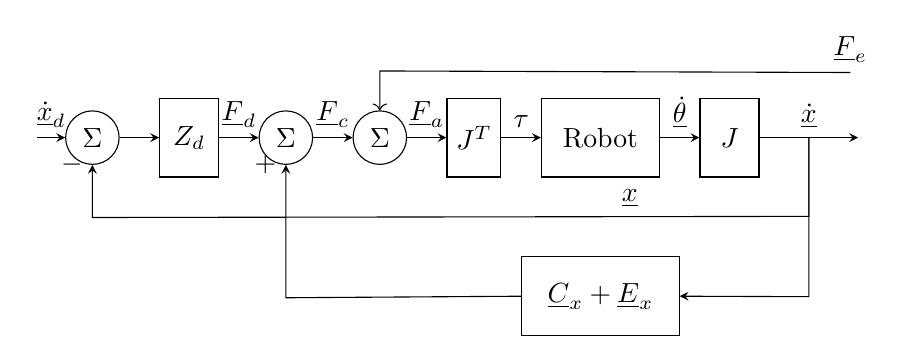
\begin{tikzpicture}
 % Sum shape
 \node[circle,draw, minimum width=0.5cm] (sum) at (-1,0){$\Sigma$} ;
 \node[draw,minimum height=1cm, minimum width=0.75cm, right=0.5cm of sum] (Zd) {$Z_{d}$};
 \node[circle, draw, 
        minimum width=0.5cm,
        right=0.5cm of Zd
        ] (sum2) {$\Sigma$};

\node[circle, draw,
    minimum width=0.5,
    right=0.5cm of sum2
    ] (sum3) {$\Sigma$};
    
% Controller
\node [draw,
    minimum width=0.5cm,
    minimum height=1cm,
    right=0.5cm of sum3
]  (JT) {$J^{T}$};
 
% System H(s)
\node [draw,
    minimum width=1.5cm, 
    minimum height=1cm,
    right=0.5cm of JT
] (robot) {Robot};

\node [draw,
    minimum width=0.75cm,
    minimum height=1cm,
    right=0.5cm of robot
    ] (J) {$J$};
    
\node [draw,
    minimum width=2cm, 
    minimum height=1cm,
    below=1cm of robot
] (model) {$\underline{C}_{x}+\underline{E}_{x}$};


\draw[-stealth] (sum3.east) -- (JT.west)
    node[midway,above]{$\underline{F}_{a}$};
    

\draw[-stealth] (sum.east) -- (Zd.west) node[midway,above](x){};
\draw[-stealth] (Zd.east) -- (sum2.west) node[midway,above](x){$\underline{F}_{d}$};
\draw[-stealth] (sum2.east) -- (sum3.west) node[midway,above](x){$\underline{F}_{c}$};

\draw[-stealth] (robot.east) -- (J.west) node[midway,above](x){$\underline{\dot{\theta}}$};

\draw[-stealth] (JT.east) -- (robot.west) 
    node[midway,above]{$\tau$};

\draw[-stealth] (J.east) -- ++ (1.25,0) 
    node[midway](output){}node[midway,above]{$\underline{\dot{x}}$};

\ExtractCoordinate{sum.west}
\draw[-stealth] (\XCoord-10, \YCoord) -- (\XCoord, \YCoord) node[midway,above]{$\underline{\dot{x}}_{d}$};
\ExtractCoordinate{sum.south}

\draw[-stealth] (output.center) -- ++ (0,-1) -- (\XCoord, \YCoord-19) node[pos=0.25,above]{$\underline{x}$} -- (sum.south) node[below,left]{$-$};

\draw[-stealth] (output.center) -- ++ (0,-2.02) -- (model.east);
\ExtractCoordinate{sum2.south}
\draw[-stealth] (model.west) -- (\XCoord, \YCoord-48) node[pos=0.25,above]{} -- (sum2.south) node[below,left]{$+$};

\ExtractCoordinate{output.north}
\draw[<-] (sum3.north) -- ++ (0, 0.5) -- (\XCoord+15, \YCoord+20) node[above] () {$\underline{F}_{e}$};
\end{tikzpicture}
\end{figure}

where
\begin{eqnarray}
 \underline{F}_{c} & = & \underline{F}_{d} + \underline{C}_{x}(\underline{\theta}, \underline{\dot{\theta}}) + E(\underline{\theta}, \underline{\dot{\theta}})\ \ \ \  \Leftarrow \text{Controller input}\nonumber \\
 \underline{F}_{a} & = & M_{x}\underline{\ddot{x}} + \underline{C}_{x}(\underline{\theta}, \underline{\dot{\theta}}) + E(\underline{\theta}, \underline{\dot{\theta}})\ \  \Leftarrow \text{Cartesian Hamiltonian dynamics} \nonumber \\
 \underline{F}_{e} &&\ \ \ \ \ \ \ \ \ \ \ \ \ \ \ \ \ \ \ \ \ \ \ \ \ \ \ \ \ \ \ \ \ \ \ \ \Leftarrow \text{Contact forces} \nonumber
\end{eqnarray}

\subsection{Actuator Dynamics}
There's a bigger problem, though, which is that we have unnoticed by you been making a major assumption through all of our control lectures, which is that you can ask your actuators to provide the forces and torques calculated by your beautiful control laws and they will just do it.

This is the vilest lie ever perpetuated by engineers on control theorists. Or maybe the reverse. It's hard to tell.

In any case: real motors and pistons don't, in fact, take ``torque'' as a command. Behind the scenes your power electronics are actually controlling current (for motors) or hydraulic flow (for hydraulic pistons) or whatever, and the folks who designed that system are only approximating when they say that current or flow is proportional to torque or force. Motors output a torque that is proportional to current via the ``motor torque constant'', which is in theory a constant (hence the name) but in practice varies by a surprisingly large amount, depending on how much you paid for the motor, how well lubricated it is, what temperature it is, how much wear it has, how well the insulation in the motor windings are holding up, how well it slept last night and whether it just had a fight with its significant other(s). We don't judge here.

Furthermore, actuators have dynamics -- motors have rotor inertia and bearing friction and all kinds of electrical current dynamics nonsense that is incomprehensible to the human mind. When we do high gain position control, we almost always ignore all of this stuff as being at worst second--order disturbance terms, because these dynamics tend to happen at frequencies well above the bandwidth of our arm, and because whatever is left over will get taken care of by our high--gain disturbance rejecting arm control.

...oh yeah. When we're doing compliance control, the bandwidth of our arm is measured in terms of force, not position, and when our arm is in contact with a stiff environment the bandwidth gets multiplied by whatever the stiffness of the least stiff mechanical component in the kinematic chain is, which can be quite high. So suddenly our arm which we thought had a 1 Hz bandwidth now has a 100 Hz bandwidth and all of those high frequency actuator dynamics aren't so high frequency anymore.

And we're \textit{also} intentionally lowered our PD gains quite a lot because we want to react to external forces. So those dynamics aren't getting rejected, like, AT ALL.

Which leads us to...
\subsection{Motor Torque Control}
Almost all the time, roboticists who implement impedance control in anger take great pains to accommodate the motor dynamics, often through directly sensing the torque the motors are putting out and trying to control that so that the upstream impedance controller mostly gets the torque it is asking for. This isn't so much hard mathematically as it is hard mechanically (because you have to sense the torque at the motor) and computationally (because this thing wants to run EVEN FASTER than the impedance control does).

One potential way to do this is to model the motor dynamics and try to cancel them. It turns out that motor dynamics, for all their weirdness, can be added into the Hamiltonian rigid body dynamics to get something that doesn't look all that scary:
\begin{eqnarray}
 M(\underline{\theta})\ddot{\underline{\theta}} + C(\underline{\theta}, \dot{\underline{\theta}}) + E(\underline{\theta}, \dot{\underline{\theta}}) & = & \underline{\tau} + DK^{-1}\dot{\underline{\tau}} + \underline{\tau}_{ext} \nonumber \\
 B\underline{\ddot{\theta}}_{m} +\underline{\tau}+DK^{-1}\dot{\underline{\tau}} & = & \underline{\tau}_{m} \nonumber \\
 \underline{\tau} & = & K(\underline{\theta}-\underline{\theta}_{m}) \nonumber
\end{eqnarray}
That last line just describes the native flexibility in the actuator and gear train, and $\underline{\theta}_{m}$ is the rotation of the motor shaft. The second line describes the actuator dynamics, e.g. the damping and rotor inertia terms.

You can try to just reject the dynamics terms using a sufficiently high gain linear control law on the motor torque, e.g.
\begin{displaymath}
 \underline{\tau}_{m} = -K_{pm}\underline{\tilde{\theta}}_{m} - K_{vm}\underline{\dot{\tilde{\theta}}}_{m} 
\end{displaymath}
which by all accounts works pretty okay, although stability is, as usually, difficult to prove. Of course, implementing this requires that you have the ability to sense or otherwise estimate $\tilde{\underline{\theta}}_{m}$, the ``tracking error'' between the actual motor position on the input side of the gear shaft and the joint angle position on the output side. This implies both a joint angle sensor (which is almost always present) and a motor shaft position sensor (which almost always isn't, unless you demand it). It also implies that you can either differentiate this signal to come up with a motor shaft velocity (pretty dicey) or build in a motor shaft rate sensor (also almost never present).

\subsection{Series--Elastic Elements (SEAs)}
One more way to handle impedance control with real actuators is to just build a mechanical compliance device into the actuator. This device will act like a lowpass filter, which will isolate the joint from the motor dynamics. It also has the nice benefit that you may not need to implement active impedance control at all: you just rely on the mechanisms in the joints to handle all that pesky business with environmental forces. So you don't need high rate control loops and so on at all, nor do you need to prove the stability of said nonexistent control loops. It's also implicitly safe, e.g. when working around humans: you aren't ever relying on software to make the robot compliant. It just \textit{is}. One notable robot family that takes this route is Robonaut and all of its descendants.

There are a couple of disadvantages with this approach. The most obvious one is that you can't get rid of that mechanical compliance when you don't want it there, for instance when you're trying to do position tracking. Another, related one is that it isn't immediately obvious how to \textit{change} the compliance when you want to perform tasks requiring different amounts of it; a third, also related one, is that this implements a joint--space compliance, not a Cartesian compliance, which is almost never what you really want.

Robonaut takes the approach of building in a nonlinear spring and two (not one) actuators per joint, because we now have two degrees of freedom per joint: one corresponding to the spring preload and one to the joint angle. In this way, you can still calculate the Cartesian--to--joint mapping in Equations \ref{stiffness}, and then preload the nonlinear springs in the joint to the calculated levels. Note that you don't necessarily get the damping in Equation \ref{damping}, though, unless you also build a mechanical damper into the joint, which to my knowledge has never been attempted.

Of course, this leads to a \textit{much} more complicated robot arm. The original Robonaut arm had 19 degrees of freedom (7 in the arm/wrist and 12 in the hand) for a total of 38 actuators (I think). In an unrelated note, the original Robonaut arm was designed by an engineer who had trained as a high--end Swiss watchmaker. The Baxter arm also takes this approach; if you've ever seen a Baxter you'll recall that Baxter arms are remarkably bulky for their length, and this is why.

It also leads to fairly complicated arm dynamics, because for the most part the mechanical compliance ion the joints manifests as an elasticity, which violates the Hamiltonian rigid--body dynamics formulations. Variations on computed torque controllers are \textit{de rigeur} for SEA--based manipulators; they typically need the extra control design effort to achieve decent free--space tracking.

\begin{thebibliography}{10}
\bibitem{hogan1985} Hogan, Neville, ``Impedance control: An approach to manipulation: Part I—Theory,'' 1985, \url{http://groups.csail.mit.edu/drl/journal_club/papers/hogan1985_applications.pdf}.

\bibitem{hogan1985II} Hogan, Neville, ``Impedance control: An approach to manipulation: Part II—Implementation,'' 1985, \url{http://groups.csail.mit.edu/drl/journal_club/papers/hogan1985_implementation.pdf}.

\bibitem{lawrence1988} Lawrence, Dale A. ``Impedance control stability properties in common implementations,'' \emph{Proceedings of the 1988 IEEE International Conference on Robotics and Automation}, IEEE, 1988.

\bibitem{hirzinger2007} Albu-Schäffer, Alin, and Ott, Christian, and Hirzinger, Gerd,  ``A unified passivity-based control framework for position, torque and impedance control of flexible joint robots,'' \emph{The International Journal of Robotics Research}, vol 26.1, pp. 23-39, 2007.

\bibitem{tomei1991} Tomei, Patrizio. ``A simple PD controller for robots with elastic joints,'' \emph{ IEEE Transactions on Automatic Control}, Vol 36.10, pp. 1208-1213, 1991.

\bibitem{lovchik1999} Lovchik, C. S., and Diftler, Myron A., ``The Robonaut hand: A dexterous robot hand for space,'' \emph{Proceedings 1999 IEEE international conference on Robotics and Automation}, (Cat. No. 99CH36288C), Vol. 2, 1999.

\bibitem{fitzgerald2013} Fitzgerald, Cliff. ``Developing Baxter,'' \emph{2013 IEEE Conference on Technologies for Practical Robot Applications (TePRA)}, 2013.
\end{thebibliography}

\end{document}
